%!TEX root = ../thesis.tex

\section{Background}
\label{sec:background}

In the introduction, the core motivation of this thesis was given which is to formally verify \glspl{isa} by model checking information flow control policies.
However, the methodology of this thesis has not been made clear.
At this point, it is not tractable to introduce this in detail.
Instead, the background of this thesis will be set up first.

The first two sections \ref{sec:verify-spec} and \ref{sec:ifc} will introduce the foundational work of \citeauthor{Reid17} \cite{Reid17} and \citeauthor{Ferraiuolo17} \cite{Ferraiuolo17}.
Following up on this, the actual subject of verification, \glspl{isa}, and the technical details of the verification process will be outlined.
There will be not only an introduction to common \glspl{isa}, especially RISC-V, (section \ref{sec:riscs}) but also to the ecosystem of processors which allows to set up a threat-model (section \ref{sec:ecosystem}).
Then, a general explanation of what model checking is will be given, concluding with the description of the nuXmv model checker that will be used in this thesis (section \ref{sec:model-checking}).

In each of these subsections , a collection of \glspl{isa} or model checkers respectively will be touched to \begin{enumerate*}[label=\alph*)]
    \item give a better feel for the field as a whole and
    \item meaningfully argue for one of the presented options to be worked with in this thesis.
\end{enumerate*}

As a final part of the background, in section \ref{sec:sum-background}, a summary of all aforementioned sections will be given which will finally allow for a outline of this thesis's methodology.

\subsection{Formal Verification of Specifications}
\label{sec:verify-spec}

As already introduced, the work of \citeauthor{Reid17} in \citetitle{Reid17} \cite{Reid17} focusses on verifying specifications, in particular \glspl{isa}, against high level properties.
The key motivation of this work is best summarized by the conclusion of the paper:
\begin{displaycquote}[p.88:22]{Reid17}
    Formal verification of programs is becoming more and more practical but, if the verification is to be meaningful, it must be based on correct architecture specifications for the hardware that the programs run on.
    That is, the specifications are a critical part of the Trusted Computing Base.
    Unfortunately, the size and complexity of architecture specifications is such that it seems inevitable that specifications will contain bugs and our previous work confirms this supposition.

    While it is common to debug specifications by \textit{testing} the specification, this paper proposes a different approach:
    we define a set of formal properties that should hold for the specification and we \textit{formally verify} the architecture specification satisfies these properties.
    We think of the relationship between the properties and the specification as being like the relationship between a nation's constitution and a nation's laws:
    the constitution is concise enough that everyone can read them while the laws are too large for effective review; the constitution can be used to test whether existing or proposed laws are compatible with high level goals; and the constitution is stable and changes very, very slowly.
\end{displaycquote}

These high-level properties comprise the formalization of \textcquote[p.88:2]{Reid17}{cross-cutting features}, i.e. features that describe expected high-level behavior of the architecture.
Cross-cutting features have the downside that they are usually hard to grasp for humans since they require a thorough understanding of the system as a whole, yet are powerful since they often (indirectly) touch many aspects of the specification.
In his paper, \citeauthor{Reid17} gives a list of requirements for such cross-cutting properties:
\begin{displaycquote}[pp.88:2-3]{Reid17}
    The central design challenge we face is to create a set of properties that:
    \begin{itemize}
        \item express the major guarantees that programmers depend on;
        \item are concise so that architects can easily review and remember the entire set of properties;
        \item are stable so that architectural extensions don't invalidate large numbers of rules;
        \item and that describe the architecture differently from existing specification to reduce the risk of common-mode failure.
    \end{itemize}
\end{displaycquote}

The aspects of the conciseness and stability of the properties implement the idea of a \enquote{constitution} for an \gls{isa} linking back to the paragraphs quoted above.
The first point, however, more plays a role for the practical applicability of the verification process.
If properties, the architecture is verified against, express \enquote{major guarantess that programmers \textins{can} depend} on, they can be used to aid in usage of the platform, e.g. by \gls{os} engineers to utilize the mechanisms of the architecture correctly and thereby to write secures \glspl{os}.
Lastly, the requirement aimed at reducing the \enquote{risk of common-mode failure} aims at combatting the downsides of other approaches to verifying specifications.
\citeauthor{Reid17} lists three commonly used ways of verifying specifications: \textcquote[p.88:2]{Reid17}{by testing specifications against existing existing implementations; by testing specifications using testsuites used to test implementations; or as a side effect of attempting to formally verify an implementation against a specification}.
These approaches, however, all face the risk of issues with the specification being undetected because the implementation and specification both are affected by the same issue, i.e. the risk of issues being undetected because of common-mode failure.
This risk can be mitigated if the properties the specification will be verified against actually expresses something \textit{new}.

\citeauthor{Reid17} applies his approach to the ARM M-Class architecture for which not only a natural language but also a machine-readable specification is available.
The machine-readable specification of the ARM M-Class architecture provides the function \asl{TopLevel} which implements the transition of the architecture from one state to another, i.e. a cycle of the processor.
The natural language specification on the other hand mainly consists of rules that constrain the behavior of the architecture in different situations, i.e. that constrain the transition relation between architectural states that implicitly is given by the \asl{TopLevel} function.

In principle, these two forms of specification also face the risk of common-mode failures.
In practice, however, it turned out that the natural language specification included several rules that described the behavior of the architecture on a very high-level thus meeting aforementioned requirements.
Using these rules as high-level cross-cutting properties, \citeauthor{Reid17} was able to find 12 bugs in the ARM M-Class specification that despite prior testing had been undiscovered up to this point.

In summary, the aspects of \cite{Reid17} that are relevant for this thesis are:
\begin{enumerate}[label=\alph*)]
    \item the paper argues for why the verification of specifications themselves is important; and
    \item the paper proposes requirements for properties to verify an \gls{isa} against.
\end{enumerate}

Additionally, the paper successfully implements its approach by partially verifying the ARM M-Class architecture.
A downside of this work, however, is that it is limited to verifying single processor transactions only.
This lies in the nature of the properties taken from the natural language specification which only constrain single transitions of the processor.

This thesis attempts to fill this gap and proposes a new way of verifying architectural specifications which will apply to multiple processor transitions.
The work in this thesis therefore also is subject to the same requirements that have been imposed on the high-level properties in \cite{Reid17}.

\subsection{Information Flow Control}
\label{sec:bg-ifc}

In \citetitle{Ferraiuolo17} \cite{Ferraiuolo17} by \citeauthor{Ferraiuolo17} the authors verify an implementation of the ARM TrustZone architecture by statically type-checking an information flow policy.
To achieve this, they enhance on the already existing \gls{hdl} language SecVerilog, extending its type system to allow more fine grained modelling of information flow policies.
Therefore, the authors verify an implementation against higher level properties as opposed verifying a specification as done by \citeauthor{Reid17} in \cite{Reid17}.
This thesis takes this general approach and lifts it to be applied to specifications rather than \glspl{hdl}.

\glspl{hdl} are very much like other, ordinary programming languages only that they are used to specify electronic circuits.
This use case introduces several novelties to \glspl{hdl} in contrast to normal programming languages, e.g. type systems are not as rich and usually comprise registers (multiple bits) and wires (one bit). i.e. they resemble much more low level systems.
In context of this thesis, think of an \gls{hdl} as a programming language with a very specific use case.

\citeauthor{Ferraiuolo17} define an \textit{information flow policy} as a lattice of security labels $ (M, \sqcup, \sqcap) $; with $ \sqsubseteq $ being the partial order on $ M $ as induced by the lattice.
Intuitively speaking, information labelled with $ a \in M $ is allowed to flow to a sink labelled with $ b \in M $ iff $ a \sqsubseteq b $, i.e. information is always allowed to flow up in the lattice but not down.

\begin{example}
    To verify an ARM TrustZone implementation, \citeauthor{Ferraiuolo17} introduce four information flow labels $ \Sigma = \{ \PT, \PU, \CT, \CU \} $ which stand for public/trusted, public/untrusted, confidential/trusted and confidential/untrusted.
    These labels form the information flow policy lattice $ (\Sigma, \sqcup, \sqcap) $ which is depicted in figure \ref{fig:sec-lattice} as a hasse diagram.
    As you can see, each of these four labels comprises two tokens from two domains of information flow control.
    The first of these domains is the one of \textit{confidentiality}, i.e. each label states that a piece of information is either public (\P{}) or confidential (\C{}).
    The second of these domains is the one of \textit{integrity}, i.e. each label states that a piece of information is either trusted (\T{}) or untrusted (\U{}) where \enquote{trusted} means whether
    the values we deal with are integrous or in other words not malicious?

    \begin{figure}
        \centering
        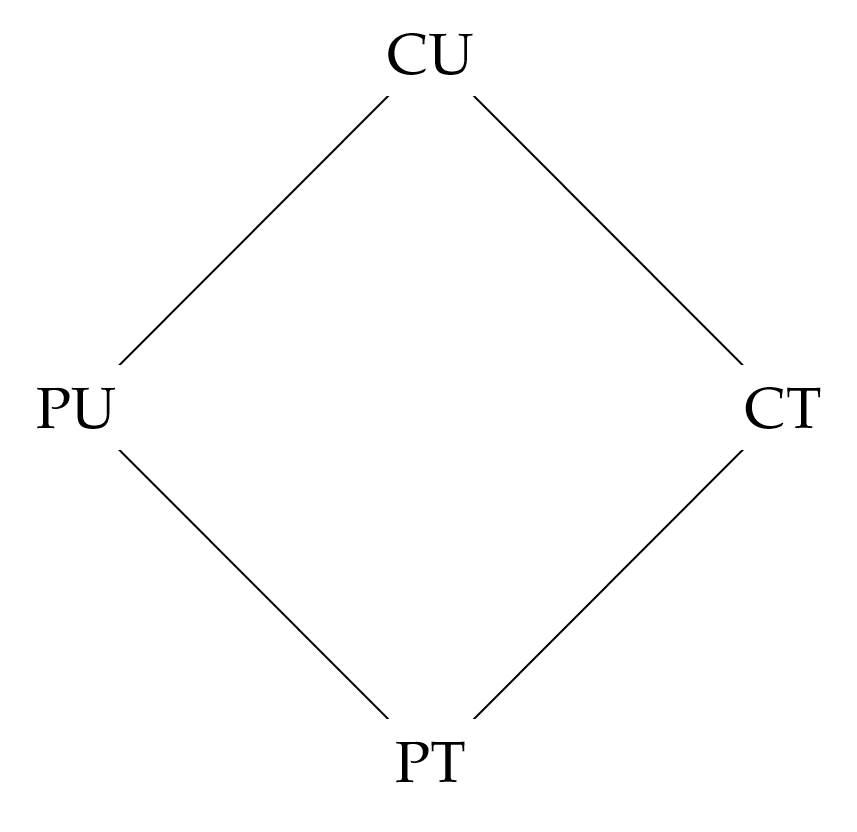
\includegraphics[width=0.4\textwidth]{figures/ifp-lattice.png}
        \caption{Security lattice for verifying an ARM TrustZone implementation \cite{Ferraiuolo17}}
        \label{fig:sec-lattice}
    \end{figure}

    It can be seen in the diagram depicting the lattice of security labels (fig. \ref{fig:sec-lattice}) that public information can flow to confidential sinks but not vice versa and that trusted information can flow to untrusted sinks but not vice versa.
    Intuitively, this means that trusted parts of the architecture must only receive trusted data and that confidential data must be handled by confidential parts of the architecture only.
\end{example}

To implement the actual \textit{control} of such an information flow policy, \citeauthor{Ferraiuolo17} introduce the \gls{hdl} language SecVerilogBL that builds upon the \gls{hdl} SecVerilog.
The core of both of these languages when it comes to information flow control is a type-system that adds syntax to the core \gls{hdl} allowing for annotating variables with security labels.
This enables verifying an information flow control policy by static type-checking.
In SecVerilog, variables are typed by labels of the respective information flow control policy.
The type of a variable is described either by a label $ l \in M $ directly, by the conjunction $ \sqcap $ or disjunction $ \sqcup $ of two labels or by a type-level function $ f $ that maps some program variable $ v $ to a type.
SecVerilogBL enhances on this by tracking security labels not only per variable but also per bit and array element therefore allowing for more fine grained annotation of the \gls{hdl} code but also adding a mechanism to downgrade information.
Since information is not allowed to flow \enquote{down} in the lattice, downgrading can be understood best as a typecast that allows such behavior.
In some \gls{hdl} programs, it might be necessary to allow for insecure flows of information (in regard to the information flow policy).
In those cases, a programmer can use \lstinline[mathescape]{downgrade(e, $ \tau $)} to annotate the expression \lstinline{e} as being of type $ \tau $, regardless of any prior annotations.
This effectively \textit{grades} the label of a bit of information \textit{down} such that information is not routed to a sink annotated with a label smaller than the information.

In total, SecVerilogBL knows seven ways to express types:
\begin{align*}
    \text{Types } \tau ::= l \mid \tau_1 \sqcup \tau_2 \mid \tau_1 \sqcap \tau_2 \mid x \mapsto \tau \mid f(x) \mid \textit{if $ e^\tau $ $ \tau_t $ $ \tau_f $} \mid \textit{case $ e^\tau $ $ \tau_1 $ \dots $ \tau_n $}
\end{align*}

As can be seen above, types are either given as simple labels of the information flow policy $ (M, \sqcup, \sqcap) $, as the disjunction or conjunction of two types, as a mapping from an index variable $ x $ to some type, as the application of some program variable $ x $ to the function $ f $ or as an $ \textit{if} $- or $ \textit{case} $-expression where $ e^\tau $ is a pure-expression, i.e. side-effect free.
Types of the form $ f(x) $ are called \textit{dependent types}.
$ e^\tau $ in $ \textit{if} $- or $ \textit{case} $- expressions might also contain program variables; if it does, these expressions also form dependent types.

Types are of a certain kind:
\begin{align*}
    \text{Kinds } k ::= l \mid \texttt{int} \rightarrow k
\end{align*}

Any type is of kind $ l $.
Furthermore, the type $ x \mapsto \tau $ is of kind $ \texttt{int} \rightarrow k $ where $ k $ is the kind of $ \tau $.
However, when type-checking is performed, types of kind $ l $ are lifted to be of kind $ \texttt{int} \rightarrow l $ such that every type is a partial function from bit indices to information flow labels.
This construct spares programmers from writing type maps for arrays and bit vectors where the type does not change per bit.
This way, a constant type $ \tau $ of kind $ l $ can be applied to a whole bit vector as for type-checking, $ \tau $ is lifted to $ i \mapsto \tau $ which is of kind $ \texttt{int} \rightarrow l $.

\begin{example}
    The following snippet shows the type annotation of parts of a register file definition in SecVerilogBL:
    \begin{lstlisting}[
        language=SecVerilogBL,
        label={snpt:reg-file},
        caption={A register file code segment \cite{Ferraiuolo17}}
    ]
        reg [0:31] {world(ns)} read;
        reg [0:31] { i -> j -> world(reg_ns[i]) } mem[0:1023];
        reg {PT} reg_ns [0:1023];
        (*\dots*)
        if(ns == 1) begin (*\label{ln:assignment}*)
            read = (reg_ns[read_addr] == 1) ?
                mem[read_addr] : 32'b0;
        end else begin
        (*\dots*)
    \end{lstlisting}

    The variables \lstinline{read} and \lstinline{reg_ns} illustrate the purpose of lifting types to higher kinds.
    Both types \lstinline{world(ns)} and \lstinline{PT} are of kind $ l $, yet they are used to annotate variables that store more than one bit.
    Because \lstinline{read} is a register with 32 bits, \lstinline{world(ns)} is lifted to \lstinline{i -> world(ns)}, i.e. each element of \lstinline{read} is of the dependent type \lstinline{world(ns)}, and since \lstinline{reg_ns} is an array of 1024 registers of width 1, \lstinline{PT} is lifted to \lstinline{i -> j -> PT}, i.e. each array element is of type \lstinline{j -> PT}, i.e. each array element's bits are of type \lstinline{PT}.

    In this example, the variable \lstinline{ns} refers to the \textit{security state} of the ARM TrustZone architecture.
    The ARM TrustZone architecture not only knows different privilege but also security states which can either be secure-state (meant to handle confidential data) or non-secure-state (meant to handle only non-confidential data).
    The variable \lstinline{ns} in the implementation of the ARM TrustZone architecture by \citeauthor{Ferraiuolo17} indicates whether the architecture currently is in secure- or non-secure-state.

    Starting in line \ref{ln:assignment}, it can be seen how dependent types work in practice.
    The function \lstinline{world} maps 0 to \lstinline{CT} and 1 to \lstinline{PU}.
    The \lstinline{if}-statement first checks whether \lstinline{ns} equals 1, in which case \lstinline{read} would be of type \lstinline{PU}.
    If \lstinline{ns} in fact equals 1, furthermore, the register \lstinline{read} shall be written with \lstinline{mem[read_addr]} but only if the type of that also is of \lstinline{PU} which is checked by ensuring that \lstinline{reg_ns[read_addr]} also equals one.
    Since each element's type of \lstinline{mem} depends on \lstinline{reg_ns}, this assignment is safe since obviously, a variable annotated with type \lstinline{PU} can be written with a value of the same type.

    If this check was omitted and \lstinline{ns == 1}, \lstinline{read} would be written with \lstinline{mem[read_addr]} when \lstinline{reg_ns[read_addr] == 0}, a variable of type \lstinline{PU} would be written with a value of type \lstinline{CT}.
    But since $ \CT \not \sqsubseteq \PU $, this would result in a type-checker error.
\end{example}

The details of this type-system are given by a collection of typing rules.
These rules are written as proofs of sequent calculus.

\begin{example}
    Consider this example of a proof written in sequent calculus:
    \begin{prooftree}
        \AxiomC{$ A $}
        \AxiomC{$ B $}
        \BinaryInfC{$ C $}
    \end{prooftree}

    This proof states that the formula $ C $ can be derived from the formulas $ A $ and $ B $ or more formally that: $ A, B \vdash C $.
\end{example}

In the context of type systems, formulas used in proofs of sequent calculus often are so called \textcquote{Ferraiuolo17}{typing judgements} where some \textit{environment} types some \textit{expression}, e.g. if $ X $ is a type environment, $ x $ an expression and $ \tau $ a type, one possible typing judgement would be $ X \vdash x : \tau $ which means that $ x $ is of type $ \tau $ under the environment $ X $.
In \cite{Ferraiuolo17} three such environments are introduced:

\begin{description}
    \item[Standard environment] $ \Gamma $ maps variables to their respective type $ \tau $.
    \item[Width environment] $ \W $ maps variables to their respective bit vector length.
    \item[Kind environment] $ \Theta $ maps types $ \tau $ to their respective kind $ k $.
\end{description}

\citeauthor{Ferraiuolo17} introduce eight typing rules; these are for constant expressions and variables, logical and arithmetic expressions, bit vector concatenation and shifting as well as array indexing.
An overview of some typing rules of \cite{Ferraiuolo17} can be found in figure \ref{fig:type-rules}\footnote{%
    It will turn out that only these typing rules are relevant in context of this thesis.
}.
The most simple type system rule probably is T-Const which types constant expressions $ n $.
These are always of type $ \bot $, i.e. \PT, and of the corresponding width $ w $.
The other type system rules share a pattern.
They assume one or two expressions ($ e $ or $ e_1 $ and $ e_2 $) to be typed in $ \Gamma; \W; \Theta $ and ensure that their corresponding types ($ \tau $ or $ \tau_1 $ and $ \tau_2 $) are of the right kind in $ \Theta $.
Then, they create a new type ($ \tau $ or $ \tau' $) and infer a type judgement for a new expression involving $ e $, $ e_1 $ or $ e_2 $ and maybe some constant $ n $.
This structure of type system rules follows the pattern of an inductive proof or inductive definition of a set where T-Const and T-Var (the typing rule for variables) are the start of induction.

When the SecVerilogBL code is being type-checked, it is verified whether all right sides of assignments are $ \sqsubseteq $-greater than the respective left sides taken together with the label of the program counter.
This means that information is only considered trusted if also the program counter can be considered to be trusted and data is considered to be confidential if either the data itself or the program counter is confidential.

\begin{figure}
    \centering
    \begin{subfigure}[t]{.5\linewidth}
        \begin{prooftree}
            \AxiomC{}
            \UnaryInfC{$ \Gamma; \W; \Theta \vdash n: \bot, w $}
        \end{prooftree}
        \caption{T-Const}
    \end{subfigure}

    \begin{subfigure}[t]{.5\linewidth}
        \begin{prooftree}
            \alwaysNoLine
            \AxiomC{$ \Gamma; \W; \Theta \vdash e_1 : \tau_1, w $}
            \UnaryInfC{$ \Theta \vdash \tau_1 : \texttt{int} \rightarrow l $}

            \AxiomC{$ \Gamma; \W; \Theta \vdash e_2 : \tau_2, w $}
            \UnaryInfC{$ \Theta \vdash \tau_2 : \texttt{int} \rightarrow l $}

            \BinaryInfC{$ \tau = i \mapsto \tau_1( i) \sqcup \tau_2(i) $}

            \singleLine
            \UnaryInfC{$ \Gamma; \W; \Theta \vdash e_1 \circ e_2 : \tau, w $}
        \end{prooftree}
        \caption{T-Logical for $ \circ \in \{ \land, \lor \} $}
    \end{subfigure}

    \begin{subfigure}[t]{.5\linewidth}
        \begin{prooftree}
            \alwaysNoLine
            \AxiomC{$ \Gamma; \W; \Theta \vdash e_1 : \tau_1, w $}
            \UnaryInfC{$ \Theta \vdash \tau_1 : \texttt{int} \rightarrow l $}

            \AxiomC{$ \Gamma; \W; \Theta \vdash e_1 : \tau_2, w $}
            \UnaryInfC{$ \Theta \vdash \tau_2 : \texttt{int} \rightarrow l $}

            \BinaryInfC{$ \tau = i \mapsto \bigsqcup_{j \in [1, i]} (\tau_1(j) \sqcup \tau_2(j)) $}

            \singleLine
            \UnaryInfC{$ \Gamma; \W; \Theta \vdash e_1 \circ e_2 : \tau, w $}
        \end{prooftree}
        \caption{T-Arith for $ \circ \in \{ +, - \} $}
    \end{subfigure}

    \begin{subfigure}[t]{.5\linewidth}
        \begin{prooftree}
            \alwaysNoLine
            \AxiomC{$ \Gamma; \W; \Theta \vdash e : \tau, w $}
            \AxiomC{$ \Theta \vdash \tau : \texttt{int} \rightarrow l $}
            \BinaryInfC{$ \tau' = i \mapsto \ite{(i < n)}{\tau(i - n + 1)}{\bot} $}

            \singleLine
            \UnaryInfC{$ \Gamma; \W; \Theta \vdash e \ll n : \tau', w $}
        \end{prooftree}
        \caption{T-LShift}
    \end{subfigure}

    \begin{subfigure}[t]{.5\linewidth}
        \begin{prooftree}
            \alwaysNoLine
            \AxiomC{$ \Gamma; \W; \Theta \vdash e : \tau, w $}
            \AxiomC{$ \Theta \vdash \tau : \texttt{int} \rightarrow l $}
            \BinaryInfC{$ \tau' = i \mapsto \ite{(i > w - n)}{\bot}{\tau(i + n)} $}

            \singleLine
            \UnaryInfC{$ \Gamma; \W; \Theta \vdash e \gg n : \tau', w $}
        \end{prooftree}
        \caption{T-RShift}
    \end{subfigure}
    \caption{A selection of typing rules for SecVerilogBL expressions \cite{Ferraiuolo17}}
    \label{fig:type-rules}
\end{figure}

In summary, the lattice of security labels taken together with the type system built on top of such a lattice implements three concepts:
\begin{itemize}
    \item A lattice $ (M, \sqcup, \sqcap) $ implements a information flow policy
    \item The typing rules implement information flow tracking
    \item Type-checking implements information flow control
\end{itemize}

\citeauthor{Ferraiuolo17} used these three concepts to verify an implementation of the ARM TrustZone architecture.
In doing so, they first implemented the architecture as a prototype and used the information flow policy to ensure that it did not contain any bugs.
Additionally, they deliberately added bugs to their implementation that have been found in other implementations of the ARM TrustZone architecture and checked whether they were able to find these bugs.
It turned out that their approach was able to detect all bugs besides those which were related to downgrading, i.e. the approach of type-checking information flow control policies gives a strong security assurances with the exception of bugs due to downgrading expressions.

In this thesis, the concept of an information flow control policy and information flow tracking will serve to define higher-level properties to verify an \gls{isa} against.
To achieve this, it must be tackled how such an information flow policy as proposed by \citeauthor{Ferraiuolo17} can be applied to \glspl{isa} such that \begin{enumerate*}[label=\alph*)]
    \item the labels can be tracked throughout the architecture by a model checker, and
    \item the policy can be controlled by the model checker.
\end{enumerate*}, i.e. how can the two concepts of information flow tracking and control be implemented using a model checker?
\todo{Do I answer above questions? -> yes, but make explicit in sec. 4}

\subsection{RISC-Architectures}
\label{sec:riscs}

\citetitle{Patterson13} defines the term \gls{isa} as follows:
\begin{displaycquote}[p.22]{Patterson13}
    One of the most important abstractions \textins{in computer design} is the interface between the hardware and the lowest-level software.
    Because of its importance, it is given a special name: the instruction set architecture, or simply architecture, of a computer.
    The instruction set architecture includes anything programmers need to know to make a binary machine language program work correctly, including instructions, I/O devices, and so on.
    Typically, the operating system will encapsulate the details of doing I/O, allocating memory, and other low-level system functions so that application programmers do not need to worry about such details.
\end{displaycquote}

Modern architectures all provide instructions of these categories: instructions for general computation, i.e. bit vector arithmetic, load-store instructions and platform management instructions.

As a target of verification, this thesis will work with \gls{risc} architectures.
In \citetitle{Hennessy12}, \gls{risc} architectures are defined by three main concepts \cite[p.C-4]{Hennessy12}:
\begin{itemize}
    \item Only load and store instructions affect or touch memory
    \item All other instructions work on registers only and always modify the full width of registers
    \item There are few instructions and their encoding is mostly homogenous
\end{itemize}

The latter aspect coined the name \textit{reduced} instruction set computer architecture.
\gls{risc} architectures are often times understood as the counterparts to \gls{cisc} architectures which describe all architectures that do not implement aforementioned \gls{risc}-properties.
The most prominent example of a \gls{cisc} architecture is the x86 architecture which is implemented by most processors manufactured by intel.

In this section, three \gls{risc} architectures will be introduced: the ARM architecture, MIPS and RISC-V.
It will turn out that these architectures can mainly be differentiated by the balance of customizability vs. feature-richness.
Whereas the RISC-V architecture is most customizable it also supports the fewest features out of the box.
On the other hand, the ARM architecture is very feature-rich but not very much customizable.
The MIPS architecture strikes a middle-ground of these two extremes.

The goal of this section is to illustrate the features and fundamental design concepts that come with contemporary \gls{risc} architectures.
The decision towards focusing on \gls{risc} architectures as a target of verification was made because their simpler approach to \glspl{isa} makes them far easier to analyze and model than \gls{cisc} processors.
Using a \gls{risc} architecture will allow for implementing an architecture in scope of this thesis while the results will still be applicable and comparable to real-world \glspl{isa} that are in use as of today.
Although choosing a \gls{risc} architecture as a target of verification already facilitates an easier implementation of the this thesis' approach, verifying a complete architecture still might be out of scope to be verified as part of a master thesis.
Introducing more than one \gls{risc} architectures will allow us to choose parts to exclude in the verification model without harming our results.

\subsubsection{Arm}

The ARM architecture knows three \textit{profiles}:
\begin{itemize}
    \item The generic \textit{application profile} ARMv8-A,
    \item the \textit{real-time profile} ARMv8-R designed for deployment scenarios in which real-time responses from a processor is crucial, e.g. in aviation,
    \item and the \textit{microcontroller} profile ARMv8-M aimed at embedded systems.
\end{itemize}

Here, the ARMv8-A profile will be put into focus.
The \citetitle{Armv8} \cite{Armv8} introduces the ARM A-class architecture as a \gls{risc} architecture with three key properties:
\begin{displaycquote}[p.A1-34]{Armv8}
    \begin{itemize}
        \item A large uniform register file.
        \item A \textit{load/store} architecture, where data-processing operations only operate on register contents, not directly on memory contents.
        \item Simple addressing modes, with all load/store addresses determined from register contents and instruction fields only.
    \end{itemize}
\end{displaycquote}

These properties already meet most of the aspects of \gls{risc} architectures as defined in \cite{Hennessy12}.
When it comes to the aspect of a homogenous instruction set, the ARM architecture makes some trade-offs on this aspect to support the three profiles available.
The ARM architecture knows three instruction sets: A64, a fixed-length 32-bit encoding instruction set for 64-bit systems, A32, a fixed 32-bit encoding length-instruction set for 32-bit systems, and T32, a variable-length instruction set that uses both 16- and 32-bit encodings to support compressed instructions.
The ARMv8-A architecture eases the challenge of correctly decoding these different instruction sets by the concept of \textit{execution states}.
The ARMv8-A supports two of these execution states: AArch64, a 64-bit execution state, and AArch32, a 32-bit execution state.
An ARM A-class processor can receive A64 instructions when in the AArch64 execution state and A32 or T32 instructions when in the AArch32 execution state.

The ARMv8-A specification defines how the processor interacts with memory which includes the specification of a cache and a memory model covering virtual addresses, memory access order control, memory access synchronization, and application level memory restrictions.
Furthermore, it is defined how processors work in a multi-processor setup and how debugging of the architecture works.
The ARMv8-A architecture also supports floating point and vector arithmetic.

If these features do not suffice for a specific use-case, there are nine optional extensions available that can be supported by an ARMv8-A processor including an extension for accelerating cryptographic tasks, for enhancing the reliability, availability and serviceability of the processor, for monitoring and profiling, for enhanced vector arithmetic, and for memory partitioning.

As for registers, the ARMv8-A architecture supports the most versatile types of registers of all \gls{risc} architectures to be compared in this thesis.
Depending on the execution state, 13 to 31 32- or 64-bit registers are supported.
Additionally, there is a \gls{pc}, a dedicated \gls{sp} and some exception link registers.
A general purpose register is used as the standard \gls{lr}.
Furthermore, there are 32 64- or 128-bit registers for floating point and vector arithmetic and a collection of \glspl{csr} that hold status information of the architecture.

\subsubsection{MIPS}

As opposed to the ARM architecture, the MIPS architecture does not only support a smaller range of registers, it also provides fewer features by standard, i.e. without extensions.
It is introduced in \citetitle{MIPS} \cite{MIPS} as: \textcquote[p.21]{MIPS}{based on a fixed-length, regularly encoded instruction set \textelp{which} uses a load/store data model, in which all operations are performed on operands in processor registers, and main memory is accessed only by load and store instructions}.
As for the aspect of a large, uniform register file, MIPS supports 32 32- or 64-bit registers the first of which is hardwired to zero, a \gls{pc} and some \glspl{csr}.
Contrary to the ARM architecture, there are no dedicated \glspl{lr} or \gls{sp}.
As indicated by the options for register width, MIPS supports both a 32- and a 64-bit architecture and instruction sets.

MIPS comes with less features out of the box than the ARM architecture; the specification only touches memory interaction including memory virtualization and cache, debugging and the interaction with a standard coprocessor that implements floating point arithmetic.
MIPS, however, is far more customizable than the ARM architecture.
Whereas in case of the latter, customizability is only given by choosing different extensions, a MIOS processor does not need to implement all features defined in the specification to be MIPS compliant.
Certain features can be left out which is called \textit{subsetting} of the architecture.
Additionally to that, MIPS allows to extend the architecture by user defined instructions, compressed instructions, enhanced media processing, enhanced geometry processing, smart card or object interaction, signal processing, multi threading, \gls{os} virtualization, vector arithmetic and an extensions aimed specifically at microcontrollers.

\subsubsection{RISC-V}
\label{sec:bg-riscv}

RISC-V was originally presented in a technical report in May 2011 \cite{RiscVISA-org} and has undergone many changes since then.
RISC-V's architectural specification is divided into two volumes: volume specifies 1 the base user-level \gls{isa} which is separated into several modules whereas volume 2 defines the privileged architecture and instruction set but still only is available as a draft.
The privileged architecture is not divided into modules but rather \textit{functional groups} that define certain aspects of privileged computing.
Such groups include for example machine- and supervisor-level \glspl{isa} and the description of a platform level interrupt controller.

This thesis works with version 2.2 of volume 1 \cite{RiscVISA} and version 1.1 of volume 2 \cite{RiscVISAP}.
RISC-V understands itself as a highly customizable architecture.
Currently, there are four variants of a base integer instruction set - one of which must be implemented by any RISC-V processor - and 13 optional extensions.
The base integer instruction sets include instructions for integer arithmetic, memory operations (loads and stores), control transfer (jumps and branches) and platform management (environment calls and status register operations).
The base integer instruction sets mainly differ in the word-size and register number.
To cope with these differences, they also make small adjustments to some functionalities but only slightly change the instruction set itself.
These four base integer instruction sets are given by:
\begin{description}
    \item[RV32I] Base integer instruction  for a 32-bit architecture
    \item[RV32E] Base integer instruction set for embedded computing
    \item[RV64I] Base integer instruction set for a 64-bit architecture
    \item[RV128I] Base integer instruction set for a 128-bit architecture
\end{description}

The RISC-V manual differentiates between standard and non-standard extensions but only introduces standard ones.
A standard extension is meant to be compatible with any other standard extension and should be \textcquote{RiscVISA}{generally useful} whilst non-standard extensions might add support for more niche use-cases and do not need to be compatible with all standard extensions.

The set of functionalities offered by standard extensions begins at quite low level with the probably most mundane being the standard extension for integer multiplication and division.
You can find a list of all standard extensions in table \ref{tbl:rv-exts}.

\begin{table}
    \centering
    \begin{tabular}{| c | l |}
        \hline
        \textbf{M} & Integer multiplication and division \\
        \textbf{A} & Atomic instructions \\
        \textbf{F} & Single-precision floating-point arithmetic \\
        \textbf{D} & Double-precision floating-point arithmetic \\
        \textbf{Q} & Quad-precision floating-point arithmetic \\
        \textbf{L} & Decimal floating-point arithmetic \\
        \textbf{C} & Compressed instructions \\
        \textbf{B} & Bit manipulation \\
        \textbf{J} & Dynamically translated languages \\
        \textbf{T} & Transactional memory \\
        \textbf{P} & Packed-SIMD instructions \\
        \textbf{V} & Vector operations \\
        \textbf{N} & User-level interrupts \\
        \hline
    \end{tabular}
    \caption{All RISC-V standard extensions}
    \label{tbl:rv-exts}
\end{table}

A subset of the RISC-V \gls{isa} is described by a so called \textcquote{RiscVISA}{\gls{isa} naming string} which comes in the following form:

\begin{grammar}
    <naming-string> ::= `RV' (`32' | `64' | `128') (`I' | `E') <extensions>
\end{grammar}

An example for a naming string is the very common \gls{isa}-subset RV64IMAFD which officially is abbreviated by RV64G.
This subset includes the integer multiplication and division, user-level interrupts, atomic instructions, single-precision and double-precision floating-point arithmetic extensions.

A RISC-V core consists of multiple \glspl{hart}.
Each \gls{hart} controls its own set of registers including a \gls{pc} and is equipped with its own instruction fetch unit.
However, multiple \glspl{hart} share the same memory.

A \gls{hart} might either control 16 or 32 general purpose registers which are named from x0 to x31.
All but one instruction sets support 32 general purpose registers whereas the exception to this is the base instruction set aimed at embedded computing, RV32E, which only supports 16 general purpose registers.

Similarly to the MIPS architecture, the first of these general purpose registers is hardwired to zero and for example can be used as a target register when the result of an instruction is not needed.
Also, there is no dedicated \gls{lr} or \gls{sp}.
RISC-V supports up to 4096 \glspl{csr}.

\subsubsection{Summary}

In the last the sections, it was shown that the ARM, MIPS, and RISC-V architectures implement the three main properties of \cite{Hennessy12} characterizing \gls{risc} architectures: a small and uniformly encoded instruction set, a large and uniform register file and a load/store architecture.
Whereas the ARM architecture supported customizability only by a list of extensions and MIPS added user defined instructions and allowed subsetting its core specification, RISC-V took the idea of customizability and made it part of the core idea of the architecture.
RISC-V supports the most simple yet fully specified processor in form of the RV32E.
It was this degree of customizability and simplicity that led to the decision to use RISC-V as a target of verification.
There are no major features RISC-V lacks in that are crucial to the concept of a \gls{risc} architecture.

\subsection{The Ecosystem of an ISA}
\label{sec:ecosystem}

\glspl{isa} are embedded in a larger context.
The goal of this thesis is to verify an \gls{isa} against higher level properties.
For this undertaking to be worthwhile, it must be clear where the limitations of these properties lie.

An \gls{isa} sits between the hardware and compilers which are utilized by programs and in particular \glspl{os}.
It serves an analogous purpose to a programming language (PL).
The latter is used by programs and \glspl{os} as a specification of the input language to compilers, the former is used by compilers as a specification of the input language to the actual hardware.
This relation is depicted in figure \ref{fig:ecosystem}.
Yet, this thesis does not verify \glspl{os}, programs, compilers or hardware.
With these boundaries in mind, it must be decided what will be incorporated in the model that will be developed over the course of this thesis.

\begin{figure}
    \centering
    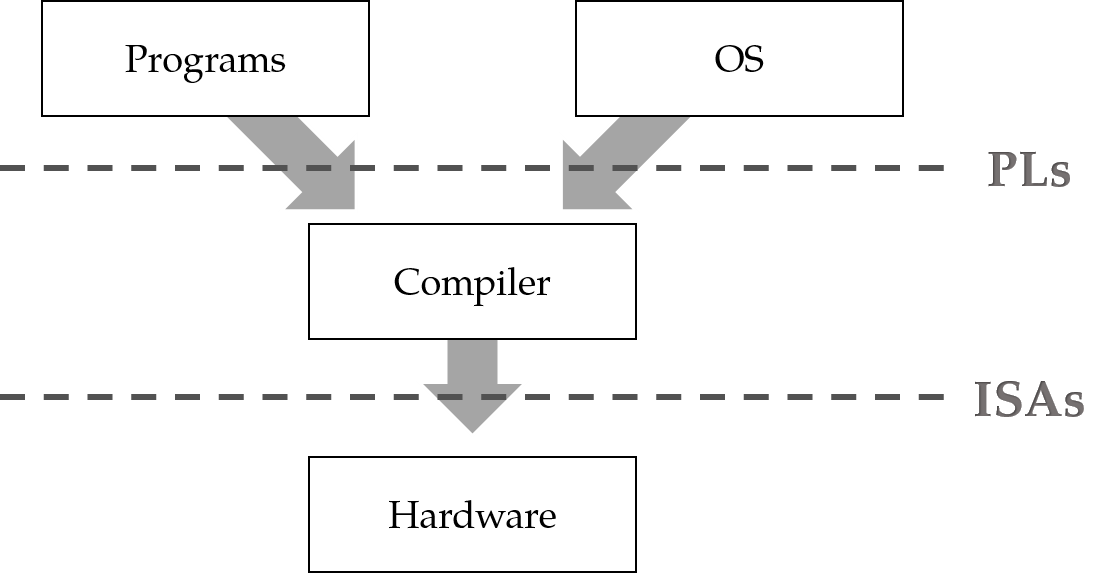
\includegraphics[width=0.7\textwidth]{figures/stack.png}
    \caption{The ecosystem of an \gls{isa}}
    \label{fig:ecosystem}
\end{figure}

\subsubsection{Microarchitectures}
\label{sec:microarchs}

When an \gls{isa} is implemented in a chip, the layout and design of this chip is often times called \textit{microarchitecture}.
Such implementations usually incorporate sophisticated features that speed up operation of the chip such as pipelining.
Instructions that are defined as part of an \gls{isa} are not atomic in regard to their execution; there usually are five steps that must be taken in order to execute an instruction (cf. \cite[p.286]{Patterson13}):
\begin{enumerate}
    \item Instruction fetch - load the instruction from memory
    \item Instruction decode and register file read - Read the fetched instruction and read registers targeted by the instruction
    \item Execution or address calculation - Use the \gls{alu} to perform the instruction or to calculate a memory address
    \item Data memory access - Access the memory for a read or write
    \item Write back - Store the result of the instruction in a register
\end{enumerate}
The microarchitecture comprises hardware modules that implement each of this steps.
To use the microarchitecture to the fullest, it is much more efficient to use these modules in a pipeline where for example after the first instruction has been fetched and handed to the module decoding it, the next instruction is fetched in parallel.
In an ideal scenario, executing $ n $ instructions using a pipeline of length $ p $ only takes $ n + p - 1 $ cycles whereas without pipelining this would take $ n * p $ cycles.

Such features introduce \textit{sub-architectural state}.
For example, pipelining introduces the \textit{state} of the pipeline which is sub-architecturally because it is independent of the \gls{isa}.
An accurate model of an \gls{isa} that aims to be true to current implementations would need to include such features.
However, since the goal of this thesis is to verify an \gls{isa}, the model to be verified must be implementation independent.
Furthermore, verifying such hardware features falls in the realm of functional correctness.
Features such as pipelining face the risk that an implementation turns out to violate the \gls{isa} because instructions might execute not as they should.
Adding to the first argument of the model not being implementation independent, including sub-architectural state into the model would lead to an indirect verification of the functional correctness of such parts, i.e. whether they truly implement the \gls{isa}.
This thesis, however, is not about verifying how pipelining can be implemented correctly but about \textit{higher level} properties of \glspl{isa}.

Additionally, aspects of the functional correctness of an implementation towards the \gls{isa} are served adequately by existing methods:
In \cite{Mukherjee16} attempts to verify hardware in general have been proposed and implementations of processors have been verified against higher level properties in \cite{Zhang15, Beatty94, Berezin98, Trippel19} or against their actual specifications in form of an \glspl{isa} in \cite{Burch94, Reid16, RISCV-formal}.

\subsubsection{Virtual Memory}
\label{sec:virtual-memory}

Virtual memory is usually managed by \glspl{os} and mostly serves two purposes: \textcquote[p.428]{Patterson13}{to allow efficient and safe sharing of memory along multiple programs \textelp{} and to remove the programming burdens of small, limited amount of main memory.}
Virtual memory is a system that replaces physical memory addresses with virtual ones.
The virtual address space usually is bigger than the physical.
Memory is divided into pages with a virtual address being made up of a page index and a page offset.
On accessing an address, the page index is translated to a physical memory address which taken together with the page offset results in the respective physical memory address.
This allows programs to treat their \enquote{personal} address space as continuous whereas in reality it comprises several pages of memory scattered all over physical memory.

Virtual memory usually is part of \glspl{isa}; e.g. the ARM architecture includes the specification of the \gls{mmu} which translates addresses and is programmed by an \gls{os} via system registers (cf. chapter D5 \cite{Armv8}).
The RISC-V specification also includes a system for managing virtual memory with an address space of 32, 39, or 48 bits (cf. section 4 \cite{RiscVISAP}).
Here, the setup of virtual memory also is delegated to an \gls{os} and can be configured by programming system registers.

Again, it is important that hardware modules that handle address translation work functionally correct.
This has been covered in \cite{Dalinger05} and will be left out in this context to keep the target of verification implementation independent.
It can be verified whether virtual memory management systems \textit{correctly} isolate programs and correctly setup virtual memory.
This problem, however, falls in the realm of \gls{os} verification and has been touched by \cite{Vaynberg12} in detail.
The reader is also referenced to the sel4 project \cite{Klein09} in which a complete kernel was formally verified.

With this research in mind, it was decided to not include virtual memory addresses in the model to be targeted for verification.
Mechanisms that provide isolation between memory regions will be modelled, however, the model does not benefit from a simulation of virtual memory addresses.
Addresses will be treated as physical ones throughout this thesis.

\subsubsection{Threat Model}
\label{sec:threat-model}

\todo{Es ist anzunehmen, dass information flow zwischen den modes stattfindet; verifiziere nicht, ob das passiert, sondern wie man das verhindern könnte}
\todo{privelege escalation vulnerabilities}

Now that two concepts that touch most architectures have been ruled out, namely sub-architectural hardware mechanisms or virtual memory, this section will give a positive description of what \textit{will} be part of the model.
This includes the question of the threat model of the higher level properties to be verified.

A key feature of modern architectures that is used by modern \glspl{os} are different privileges levels.
For example, the RISC-V architecture supports up to three different privilege levels; from lowest to highest: user-mode, supervisor-mode and machine-mode.
Higher privilege levels usually give access to more system control registers, specific instructions and often times work hand in hand with specific semantics of system registers, e.g. RISC-V supports physical memory regions which support settings for each privilege level, i.e. certain regions of physical memory can be set readable to machine- but not user-mode, etc.

In a sense, privilege modes play a similar role to virtual memory.
Both concepts are used by \glspl{os} in very fundamental ways and therefore are relevant for the security of a system as a whole.
Yet, hardware only supports the foundation for virtual memory, i.e. address translation and the possibility to set properties of memory regions, whereas privilege levels and interrupts are systems offered to the \gls{os} and implemented in the hardware completely.
\glspl{os} use memory management systems to offer virtual memory to applications but rely on privilege levels to function at all.
While it was argued that verification of virtual memory systems should be targeted at \glspl{os} the same can not be said for the verification of privilege levels.
Thus, this thesis will focus on the mechanics of privilege levels in the process of verification.

This links back to \cite{Reid17}; recall that one goal of this work was to \textcquote[p.88:2]{Reid17}{express the major guarantess that programmers depend on}.
Since \glspl{os} heavily rely on correct implementations of privilege levels and especially the mechanics to transition between those, it is of specific interest to verify high level properties about the workings of these mechanisms which will lead tp insights in these guarantees.

Privilege levels go hand in hand with interrupt and/or exception handling.
Interrupts generally are used in \glspl{isa} to transfer control to specific privilege modes and/or programs, e.g. whenever you press a key on your keyboard, a keyboard interrupt is generated that is handled by the appropriate device driver and propagated by the \gls{os} to the correct application, e.g. your text editor or shell.
Exceptions usually refer to error conditions that arise during computation.
For example, coming back to physical memory regions in RISC-V, if user-mode would attempt to read from a region unreadable to it an exception would be generated.
It is the obligation of software running in machine-mode to handle such error conditions - usually related software comes as part of an \gls{os}.

To put the mechanics of transitions between privilege levels to a test, the threat model taken as a basis of the verification process in this thesis is the following\footnote{%
    Since the decision to work with RISC-V in this thesis has already been made, the threat model was be phrased with this in mind.
}:
\begin{quote}
    Assume that user-mode has been completely compromised.
    Is there any way it can gain access to secret data handled by machine-mode or it can gain control over machine-mode?
\end{quote}

Intuitively, linking privilege modes back to \glspl{os}: Assume you have a malicious app on your computer.
Is there any way it can use the \gls{isa} that is built into your computer to either access secret data or hijack your \gls{os}?

This goes beyond what can be verified purely in terms of hardware verification as discussed in section \ref{sec:microarchs}.
Even if it could be assumed that the hardware your computer is running on accurately implements the respective \gls{isa} - as long as the design of that \gls{isa} is flawed in the sense that it has security holes baked into it, i.e. into the \gls{api} that is used by the \gls{os} to give instructions to the hardware, there is no hope for secure systems\footnote{%
    Research verifying hardware against higher-level properties has been discussed in section \ref{sec:microarchs}.
    Without going into details on this research, the approach of this thesis still is an important addition to this research as it is more general, i.e. implementation independent whereas hardware verification by its very nature is implementation dependent.
}.

\todo{Give reference and reasoning}
In this threat model, timing channels are excluded.

\subsection{Model Checking}
\label{sec:model-checking}

Model checking is a technique that falls into the domain of formal verification.
It is one way to prove that a given system complies with a given specification.
\citeauthor{Baier08} introduce model checking in their book \citetitle{Baier08} \cite{Baier08} as:
\begin{displaycquote}[p.7ff.]{Baier08}
    \textit{Model-based} verification techniques are based on models describing the possible system behavior in a mathematically precise and unambiguous manner. \textelp{}
    This provides the basis for a whole range of verification techniques ranging from an exhaustive exploration (model checking) to experiments with a restrictive set of scenarios in the model (simulation), or in reality (testing). \textelp{}

    Model checking is a verification technique that explores all possible system states in a brute-force manner.
    Similar to a computer chess program that checks possible moves, a model checker, the software tool that performs the model checking, examines all possible system scenarios in a systematic manner.
    In this way, it can be shown that a given system model truly satisfies a certain property. \textelp{}

    Typical properties that can be checked using model checking are of a qualitative nature:
    Is the generated result OK?,
    Can the system reach a deadlock situation, e.g., when two concurrent programs are waiting for each other and thus halting the entire system?
    But also timing properties can be checked:
    Can a deadlock occur within 1 hour after a system reset?, or, Is a response always received within 8 minutes?
\end{displaycquote}

Model checking therefore deals with two parts: Firstly, a model of some system, secondly, properties formalized on the basis of some specification.
Systems to be model checked come in many forms.
They range from software libraries over hardware designs to embedded controllers.
The same is true for specifications.
Those can be fully fledged \textit{actual} specifications that describe the requirements to a system exhaustively or higher level properties that generally should apply to systems such as deadlock freeness as mentioned in \cite{Baier08}.

More technically, in model checking some system is taken and transformed into a model using a formal language like PROMELA (cf. section \ref{sec:spin}) and a specification is taken and transformed into a property usually expressed in some formal logic, e.g. \gls{ltl}.
Then it is verified via a model checker whether the system model models the formal property.
Note that \enquote{model} in this context is ambiguous.
One the one hand this term refers to the model of the system as a simplified description.
On the other hand, this term refers to the logical models-relation $ \models $ which is actually being checked.

An overview of model checking is given in figure \ref{fig:model-checking}.
There, the idea and purpose of model checking is depicted.
In summary, model checking is a technique that allows to solve the problem of ensuring that a system complies with a specification.
By translating the system into a model and the specification into a formal property this problem can be translated into \textit{checking} whether the model \textit{models} the formal property.

\begin{figure}
    \centering
    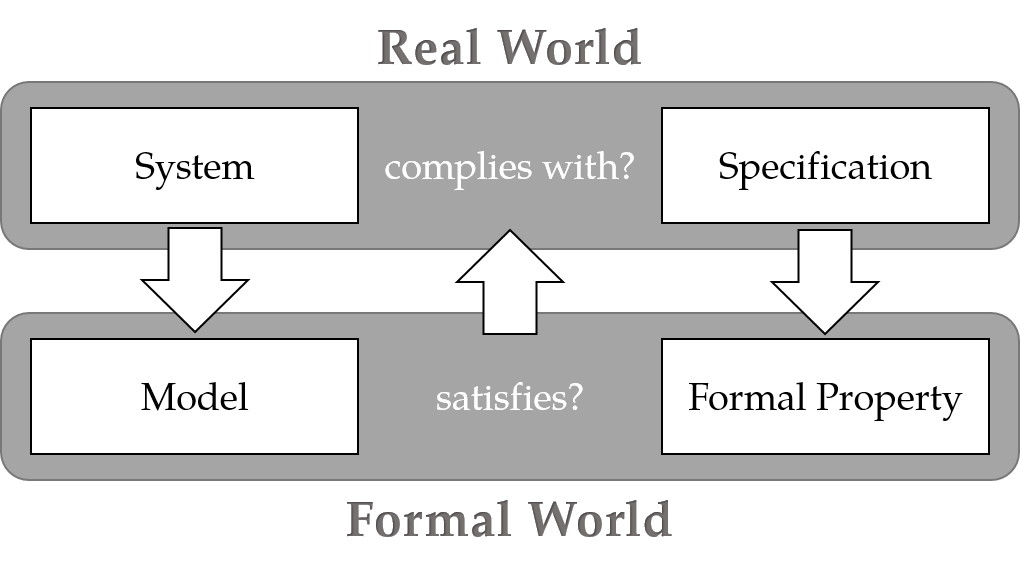
\includegraphics[width=0.7\textwidth]{figures/model-checking.png}
    \caption{Overview of Model Checking}
    \label{fig:model-checking}
\end{figure}

It has already been mentioned in the introduction of both the thesis as a whole and this section that the model checker to be used in this thesis is nuXmv.
The aim of this subsection is to introduce nuXmv and two other tools that were taken into consideration for this thesis.
These other two model checkers are called SPIN and SPACER.
By introducing three model checkers, we want to give a feel for all the different flavors of model checkers and be able to argue for why nuXmv was chosen over others.
However, this section does not intend to perform an thorough analysis of contemporary model checkers.

\subsubsection{SPIN}
\label{sec:spin}

SPIN (which stands for \textit{S}imple \textit{P}romela \textit{IN}terpreter) is a model checker which has been originally developed by Bell Labs and made freely available since the nineties.
As its name suggests, it uses PROMELA as input language.
\textit{The Spin Model Checker: Primer and Reference Manual} which has been used as source for this section, describes SPIN initially as follows:
\begin{displaycquote}[p.1]{SpinManual}
    SPIN can be used to verify correctness requirements for systems of concurrently executing processes.
    The tool works by thoroughly checking either hand-built or mechanically generated models that capture the essential elements of a distributed system's design.
    If a requirement is not satisfied, SPIN can produce a sample execution of the model to demonstrate this.
\end{displaycquote}

As indicated by the quote, SPIN focusses heavily on the verification of distributed or parallel systems.
This is reflected not only in its input language but also in the way how properties are expressed.
For an introduction by example to PROMELA, cf. snippet \ref{snpt:spin-exm}.
PROMELA relies on describing systems as sets of processes that run in parallel where parallel means that each process can advance its state (generally) independent of other processes\footnote{%
    We added the restriction \textit{generally} to the claim because processes can be set up such that they deliberately wait for other processes to send them a message or set some shared state accordingly.
    However, such mechanisms where processes depend on each other always need to be implemented accordingly.
}.

In snippet \ref{snpt:spin-exm}, two processes of the same type \lstinline{user} are declared in line \ref{ln:proc}.
The idea of this snippet is to implement and verify an algorithm that grants these two processes mutually exclusive access to the critical region spanning lines \ref{ln:crit-start}-\ref{ln:crit-end}.
This is ensured by the assertion in line \ref{ln:assert} since variables in SPIN are always initialized to 0 - if two processes had access to the critical region at the same time, \lstinline{cnt} would become 2 at some point.

The details of the protocol implemented in lines \ref{ln:excl-start}-\ref{ln:excl-end} are not relevant for this thesis.
Their purpose is to grant mutual exclusive access to the critical region.
However, this part of code gives you an indication for how models written in PROMELA look like.
Besides \lstinline{if} statements and labels similar to those in C (cf. line \ref{ln:label}), PROMELA supports \lstinline{do}-loops to control process execution flow.
\lstinline{do}-loops run indefinitely until they are exited manually by a \lstinline{break} statement.

As data types, PROMELA knows three categories: processes, message channels and data objects.
Data objects comprise atomic data types such as \lstinline{byte}, \lstinline{bool}, \lstinline{int}, etc. as well as complex data type defined by \lstinline{typedef} that define a complex structures that have fields of data objects.
Both atomic data types and complex data types are very close to the data types of C.

\begin{figure}
    \begin{lstlisting}[
        caption={Faulty Mutual Exclusion Algorithm Implemented in PROMELA \cite{SpinManual}},
        label={snpt:spin-exm}
    ]
        byte cnt;
        byte x, y, z;

        active [2] proctype user() (*\label{ln:proc}*)
        {
            byte me = _pid + 1;
        again: (*\label{ln:label}*)
            x = me; (*\label{ln:excl-start}*)
            if
            :: (y == 0 || y == me) -> skip
            :: else -> goto again
            fi;

            z = me;
            if
            :: (x == me) -> skip
            :: else -> goto again
            fi;

            y = me;
            if (z = me) -> skip
            :: else -> goto again
            fi; (*\label{ln:excl-end}*)

            cnt++; (*\label{ln:crit-start}*)
            assert(cnt == 1); (*\label{ln:assert}*)
            cnt--; (*\label{ln:crit-end}*)
            goto again
        }
    \end{lstlisting}
\end{figure}

Snippet \ref{snpt:spin-output} shows the output when verifying snippet \ref{snpt:spin-exm} with SPIN where it is assumed that latter snippet was written into a file called \lstinline{mutex_flaw.pml}.
The lines of the output are structured as follows: at the beginning of each line, a step index indicating the progress of all processes can be seen, whilst \lstinline{proc X (NAME)} indicates the process that has made progress by its ID and name.
The rest of the line \lstinline{line X ... [CODE]} shows the code executed by the process along with the corresponding line number in the source file\footnote{%
    In this case, line numbers don't fully align with snippet \ref{snpt:spin-exm} but this is not relevant here.
}.
Notice, how processes 0 and 1 progress completely independent from each other, executing code on a line by line basis where each step of any process counts as a state transition of the whole model.

\begin{figure}
    \begin{lstlisting}[
        caption={SPIN Example Output \cite{SpinManual}},
        label={snpt:spin-output}
    ]
        1:  proc    1 (user) line   5 ... [x = me]
        2:  proc    1 (user) line   8 ... [(((y==0) || (y==me)))]
        3:  proc    1 (user) line  10 ... [z = me]
        4:  proc    1 (user) line  13 ... [((x = me))]
        5:  proc    0 (user) line   5 ... [x = me]
        6:  proc    0 (user) line   8 ... [(((y==0) || (y==me)))]
        7:  proc    1 (user) line  15 ... [y = me]
        8:  proc    1 (user) line  18 ... [((z = me))]
        9:  proc    1 (user) line  22 ... [cnt = cnt+1]
        10: proc    0 (user) line  10 ... [z = me]
        11: proc    0 (user) line  13 ... [((x = me))]
        12: proc    0 (user) line  15 ... [y = me]
        13: proc    0 (user) line  18 ... [((z==me))]
        14: proc    0 (user) line  22 ... [cnt = (cnt+1)]
        spin: line 223 of "mutex_flaw.pml", Error: assertion violated
        spin: text of failed assertion: assert((cnt==1))
        15: proc    0 (user) line  23 ... [assert((cnt==1))]
        spin: trail ends after 15 steps
        # processes: 2
            cnt = 2
            x = 1
            y = 1
            z = 1
        15: proc    1 (user) line  23 "mutex_flaw.pml" (state 20)
        15: proc    0 (user) line  24 "mutex_flaw.pml" (state 21)
        2 processes created
    \end{lstlisting}
\end{figure}

Assertions, however, are not the only way to express properties of PROMELA models for SPIN.
Furthermore, there are:
\begin{itemize}
    \item Labels
    \item Never claims
    \item Trace assertions
\end{itemize}

Labels have already been introduced informally along with snippet \ref{snpt:spin-exm}.
To express properties about a model, certain types of labels can be used to give semantics to process state.
For example, you can label a certain part of process code as and end-state that might look like an idling-state to SPIN by default.
Idling- and end-states are important to SPIN when it's checking for deadlock-freeness of systems.
By default, if all processes are in an idling-state and wait for some kind of signal, this state is considered to be a deadlock.
However, in some situations it might be perfectly fine for some of the processes to idle in a specific state which should not contribute towards deadlocks.
Labeling parts of code as end-state contributes towards this.

Never claims are processes themselves.
They run like any other process but must not terminate otherwise they're regarded as failure.
This is the most complex way to express properties and in fact falls together with writing \gls{ltl} properties about a model which will be introduced in section \ref{sec:nuxmv}.
Therefore SPIN also allows to express such never properties in \gls{ltl} directly via their command line interface.

The last type of properties, trace assertions, solely deal with message passing and therefore are not relevant to this thesis.

For some, it might be obvious at this point why we decided against using SPIN as the model checker of this thesis.
Its focus on verifying distributed and parallel systems is obvious and would make implementing an \gls{isa} in it very hard.
In the \textit{Primer and Reference Manual} for SPIN it is written:
\begin{displaycquote}[p.33]{SpinManual}
    \textins{W}e saw that the emphasis in PROMELA models is placed on the coordination and synchronization aspects of a distributed system, and not on its computational aspects. \textelp{}
    The specification language we use for systems verification is therefore deliberately designed to encourage the user to abstract from the purely computational aspects of a design, and to focus on the specification of process interaction at the system level.
\end{displaycquote}

However, the \gls{isa} we will attempt to verify
\begin{enumerate*}[label=\alph*)]
    \item will most likely not include components \enquote{interacting at the system level} and
    \item will be verified on a component level, i.e. computationally as well - even in the case where multiple system level components would be given.
\end{enumerate*}

Furthermore, it is unreasonable to assume that an implementation of instructions of an \gls{isa} could be implemented in a single statement of PROMELA.
Yet, this should be the goal as otherwise as shown in snippet \ref{snpt:spin-output} what is regarded as state by SPIN would not fall together with what is regarded as state in an \gls{isa}.
For an \gls{isa}, you typically would consider the \textit{state} of registers and memory to be the state of the \gls{isa} whilst some instruction advances this state.
However, for SPIN more complex state transitions would result in us not being able to differentiate architectural states of the \gls{isa} natively since the process implementing the \gls{isa} would change state on each line of code executed.
This could be circumvented by using the \lstinline{atomic} keyword offered by PROMELA which lets you wrap a group of PROMELA statements such that they're considered as one atomic statement that advances the process state only by one step.
However, this would lead to a model consisting of one process all of its code being wrapped by one \lstinline{atomic} statement.
This would massively contradict the key idea of SPIN of simple models being \textit{abstracted} from computationally complex code.
In this case, we'd have skipped the whole step of abstracting from some computational model that has distributed components running in parallel.
Not only could this lead to performance issues, it also can be safely assumed that the work for this thesis would be cumbersome and might stumble over obstacles induced by abusing SPIN.

\subsubsection{\muZ{} \& SPACER}
\label{sec:spacer}

\muZ{} is a Datalog-engine that provides querying fixed points with constraints and has been proposed in \cite{Hoder11}.
According to \textit{An Introduction to Database Systems} \cite[p.790ff]{Date00}, Datalog is a descriptive and querying language that originated in the field of database management systems.
At its core, Datalog programs are sets of \textit{rules} that combine predicates only using variables and constants to Horn-clauses, i.e. disjunctions with one positive literal at maximum.
For example, consider the following rule $ \pi_0 $ which expresses the transitivity of a predicate $ P $:
\begin{equation*}
    \pi_0 := P(a, b) \land P(b, c) \Rightarrow P(a, c)
\end{equation*}
Such programs are then used to \textit{deduct} facts from the set of rules.
To illustrate what this means, we introduce two other rules.
\begin{align*}
    \pi_1 := & P(0, 1) \Rightarrow \top \\
    \pi_2 := & P(a, b) \Rightarrow P(a + 1, b + 1)
\end{align*}
The Datalog-program $ \Pi := \{ \pi_0, \pi_1, \pi_2 \} $ now induces the relation $ < $ on all natural numbers including $ 0 $.
$ \pi_1 $ sets up a start of induction which, stating that $ 0 $ is smaller than $ 1 $.
This is generalized for all natural numbers by $ \pi_2 $.

Whether or not this exact Datalog-program is supported by a given Datalog-engine depends on the extensions implemented by the respective engine.
Our example relies on an extension for scalar operators since we use the $ + $ operator.

As briefly mentioned, Datalog also supports queries.
Datalog queries comprise only one predicate and a special head $ ? $.
\begin{equation*}
    q_0 := P(0, x) \Rightarrow \; ?
\end{equation*}
The result to a query is the set of all values for each variable that make the predicate true.
In this case, the result set would be $ \{ 1, 2, 3, \dots \} $.
If no variables but only constants are given in the query, Datalog simply determines whether the given predicate can be derived for the given constants.

\muZ{} now is a Datalog-engine that comes as part of the SMT solver z3 \cite{Moura08} and adds support for expressing Horn-clauses to it.
For example, consider the implementation of the program $ \Pi $ for \muZ{} as depicted in snippet \ref{snpt:muz-exm}.
This example yields \smt{sat} as result when executed, meaning, that \smt{goal} can be derived from the rules at hand.

\begin{figure}
    \begin{lstlisting}[
        language=SMT2,
        caption={Implementation of $ \Pi $ for \muZ{}},
        label={snpt:muz-exm}
    ]
        (declare-var a Int)
        (declare-var b Int)
        (declare-var c Int)

        (declare-rel ge (Int Int))
        (declare-rel goal ())

        (rule (ge 0 1))                     ; pi_1
        (rule (=>   (ge a b)                ; pi_2
                    (ge (+ a 1) (+ b 1))))
        (rule (=>   (and (ge a b) (ge b c)) ; pi_0
                    (ge a c)))

        (rule (=>   (ge 10 15)
                    goal))
        (query goal)
    \end{lstlisting}
\end{figure}

SPACER \cite{Komuravelli13} is an algorithm that combines two widely implemented approaches of currently available formal verification tools: \gls{2bmc} and \gls{cegar}.
In its implementation, SPACER uses \muZ{} as a backend.
The paper describes those techniques as follows:
\begin{displaycquote}[p.1f]{Komuravelli13}
    The key idea of \gls{2bmc} is to iteratively construct an under-approximation \textins{(or refinement)} $ U $ of the target program $ P $ by unwinding its transition relation and check whether $ U $ is safe using \gls{bmc}.
    If $ U $ is unsafe, so is $ P $.
    Otherwise, a proof $ \pi_U $ is produced explaining \textit{why} $ U $ is safe.
    Finally, $ \pi_U $ is generalized (if possible) to a safety proof of $ P $.
    \textelp{}

    Thea idea of \textins{\gls{cegar}} is to iteratively construct, verify, and refine an abstraction (\textit{i.e.}, an over-approximation) of $ P $ based on abstract counterexamples.
\end{displaycquote}

The key to understanding how SPACER works is to understand what under- or over-approximation of programs are.
For the sake of brevity, these concepts will be introduced by example.
Consider the program $ P $ as depicted in snippet \ref{snpt:spacer-p}.
$ P $ performs an integer division with remainder for a natural number \lstinline{n} by a divisor \lstinline{div} storing the results in \lstinline{ratio} and \lstinline{mod}.
Intuitively speaking, $ \hat{P} $ is an under-approximation (or abstraction) of $ P $ if for every part of $ P $ there is a corresponding part of $ \hat{P} $ whose effects are logically entailed by the original part.
Vice versa, $ P $ is an over-approximation of $ \hat{P} $.
An example for an over-approximation of $ P $ in snippet \ref{snpt:over-p} and an example for an under-approximation of in snippet \ref{snpt:under-p}.
For abstracting $ P $ to $ \hat{P} $ a couple of lines were removed whilst all other were left untouched.

\begin{figure}
    \centering
    \begin{minipage}{.45\linewidth}
        \begin{lstlisting}[
            linewidth=0.9\linewidth,
            caption={Program $ P $},
            label={snpt:spacer-p}
        ]
            n = abs(input());
            div = abs(input());
            ratio = 0;
            mod = 0;
            n = n - div;
            while (0 <= n) {
                ratio++;
                n = n - div;
            }
            mod = div + n;
        \end{lstlisting}
    \end{minipage}

    \begin{minipage}[t]{.45\linewidth}
        \begin{lstlisting}[
            linewidth=0.9\linewidth,
            caption={Refinement $ \bar{P} $},
            label={snpt:under-p}
        ]
            n = abs(input());
            div = abs(input());
            ratio = 0;
            mod = 0;
            n = n - div;
            if (0 <= n) {
                ratio++;
                n = n - div;
                if (0 <= n) {
                    (*\dots*)
                }
            }
        \end{lstlisting}
    \end{minipage}\hspace{0.1\linewidth}%
    \begin{minipage}[t]{.45\linewidth}
        \begin{lstlisting}[
            linewidth=0.9\linewidth,
            caption={Abstraction $ \hat{P} $},
            label={snpt:over-p},
            showlines=true
        ]
        n = abs(input());
        div = abs(input());
        ratio = 0;
        mod = 0;

        while (0 <= n) {

            n = n - div;
        }

        \end{lstlisting}
    \end{minipage}
\end{figure}

With this example at hand it can more easily be seen how \gls{2bmc} and \gls{cegar} relate to under- and over-approximations respectively.
Assume that we want to prove that always \lstinline{0 <= ratio}.
In the case of the refinement $ \bar{P} $ in snippet \ref{snpt:under-p} we could follow the idea of \gls{2bmc} and iteratively check whether \lstinline{0 <= ratio} for finite traces of $ P $.
If a counterexample is found in $ \bar{P} $ it is obvious that this counterexample must also apply to $ P $.
However, if no counterexample is found but a proof for the property at hand can be constructed one can only hope that this proof can be generalized to $ P $.

On the other hand, the converse holds for over-approximations, i.e. abstractions.
If a property is checked for the abstraction $ \hat{P} $ of $ P $ and a positive result in form of a correctness proof is given this proof will apply to $ P $ as well.
However, when a counterexample is given, it is unclear whether it applies to $ P $.
If the counterexample does not apply to $ P $, the idea of \gls{cegar} \cite{Clark00} applies which is to refine the abstraction at hand in such a way that the counterexample does not apply to it anymore and re-iterate on the verification process.

SPACER uses both of these techniques to prove safety properties of programs expressed in Datalog using \muZ{}.
These safety properties are expressed using custom relations in Datalog such as \smt{goal} in snippet \ref{snpt:muz-exm}.
SPACER then tries either to construct a proof why the property at hand cannot be derived from the axioms of the Datalog program or it gives a counterexample illustrating a possible weakness of the program.
In theory, Datalog could be used for the implementation of this thesis.
A single predicate could be used to simulate the architectural state of the instruction set architecture at hand whilst each instruction could be modelled via a separate rule.

However, whereas the limiting factor for SPIN was the modelling language, the limiting factor for SPACER is the output of the tool.
In case of a property failing to be verified, no counterexamples are given but SPACER simply outputs there is an trace of the program for which a given property does not hold but without specifying the trace itself.
\muZ{} itself can be configured to give a more detailed result however this would still not include a \textit{trace of derivations}.
For SPACER or \muZ{} to be usable in the context of this thesis, these tools would need to output a log of variable values or steps taken when applying rules.

\subsubsection{nuXmv}
\label{sec:nuxmv}

nuXmv \cite{Cavada14} is a symbolic model checker that is able to model check invariants, \gls{ltl} and \gls{ctl} formulas.
Symbolic model checkers have been introduced in \cite{Burch92} and encode the state-space of the system to model check in \glspl{bdd} which work analogously to binary decision trees with the major difference that \glspl{bdd} are not trees but directed, acyclic graphs.

nuXmv supports both finite and infinite state transition systems.
These systems are expressed in the form of \textit{modules}.
At its heart, a module consists of a collection of variables, \smv{INIT} (i.e. initial) constraints and \smv{TRANS} (i.e. transition) constraints.
There are more syntactical constructs, e.g. macros or constants, but these do not add to the expressiveness of nuXmv but either serve as syntactic sugar or enhance on performance if used.
A module in nuXmv induces a set of state transition systems.
The state space of such a system is given by the variables of the module, i.e. an assignment to all variables is a state of the system.
The initial state must model the \smv{INIT} constraints the transition relation must model the \smv{TRANS} constraints.
Whenever nuXmv checks a property $ P $ for a module $ M $ it is checked if every state transition system $ S $ which is given by $ M $ models $ P $.

The input language to nuXmv is strongly typed.
Variables can be of type boolean, integer range, a custom enumeration, bit vector or array in the case of finite state transition systems or additionally integers and reals which induce infinite state transition systems.
\smv{INIT} constraints are simple formulas of propositional logic supporting standard expression to deal with bit vectors, arrays, etc., such as basic arithmetic, array indexing, standard boolean operators on both bit vector and boolean level, but also case and if-then-else expressions.
\smv{TRANS} constraints also are forumlas of propositional logic but additionally support use of the \smv{next(...)} operator which is a reference to the value of the respective expression in the next state.

\begin{example}
    Consider the example module depicted in snippet \ref{snpt:nuxmv} modeling a pair of traffic lights; one for pedestrians crossing the street, the other for cars driving on the street.

    \begin{figure}
        \begin{lstlisting}[
            language=smv,
            caption={An example of a nuXmv module},
            label={snpt:nuxmv}
        ]
            MODULE main
                IVAR
                    ped_button : boolean;
                VAR
                    ped_waiting : boolean;
                    traffic_lights : { r, g };
                    ped_lights : { r, g };

                INIT traffic_lights != ped_lights;
                ASSIGN
                    init(ped_waiting) := FALSE;
                    next(ped_waiting) :=
                        (ped_lights = g ? FALSE : ped_waiting | ped_button);
                    next(ped_lights) :=
                        (ped_waiting ? g : r);
                    next(traffic_lights) :=
                        (next(ped_lights) = g ? r : g);
        \end{lstlisting}
    \end{figure}

    This module uses an \smv{IVAR} - \textit{input variable} - declaration; a language construct that hasn't yet been introduced.
    Input variables have the characteristic that they are \enquote{read-only}.
    Technically, every variable is read-only since they can not be assigned directly but only constrained.
    \smv{IVAR} variables, however, are \enquote{read-only} because they cannot be used in \smv{INIT} constraints or inside \smv{next(...)} expressions.
    In other words, the transition of input variables appears to be completely random as it is completely unconstrained and as such can take any value in any step.
    In this case, the input variable to the module signals whether a pedestrian just pressed the button indicating the desire to cross the road.

    Furthermore, the module comprises three ordinary variables: the boolean variable \smv{ped_waiting} which indicates whether a pedestrian is waiting to cross the road as well as \smv{traffic_lights} and \smv{ped_lights} modelling the traffic or pedestrian lights and both are of an enum type that contains the symbols \smv{r} for red and \smv{g} for green.

    Then, there is one \smv{INIT} constraint asserting that one of the traffic lights is green and the other is red at startup.
    All other constraints are expressed in the \smv{ASSIGN} statement which is syntactic sugar for a group of \smv{INIT} or \smv{TRANS} statements.
    Its semantics should be clear from the example.
    \smv{ped_waiting} is initialized to \smv{FALSE} and becomes false after the traffic lights switched to green; otherwise it can become \smv{TRUE} whenever the input variable \smv{ped_button} happens to be \smv{TRUE}.
    The pedestrian lights switch to green whenever some pedestrian is waiting and otherwise switch to red, the traffic lights are coupled to the pedestrian lights and become red whenever the pedestrian lights are green and become green otherwise.
\end{example}

nuXmv supports four types of specifications: invariants, \gls{ltl} or \gls{ctl} formulas, and \gls{psl} expressions.
Here, an introduction into \gls{psl} will be skipped since \gls{psl} is directly aimed at hardware verification (cf. \cite{Foster05}).

Invariants are the simplest form of specification and can also be expressed in both, \gls{ltl} and \gls{ctl}.
In the context of nuXmv, an invariant is formally given by a next-expression, i.e. an expression that can contain the use of the \smv{next} operator.
Invariants specify that something (i.e. the respective next-expression) must be true in all reachable states of a model.

\begin{figure}
    \def\subfigw{0.5\textwidth}
    \def\figscale{0.4}
    \begin{subfigure}[b]{\subfigw}
        \centering
        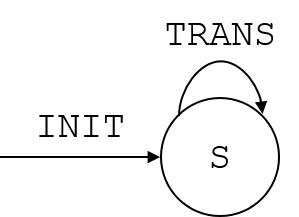
\includegraphics[scale=\figscale]{figures/module.png}
        \caption{nuXmv module}
    \end{subfigure}
    \begin{subfigure}[b]{\subfigw}
        \centering
        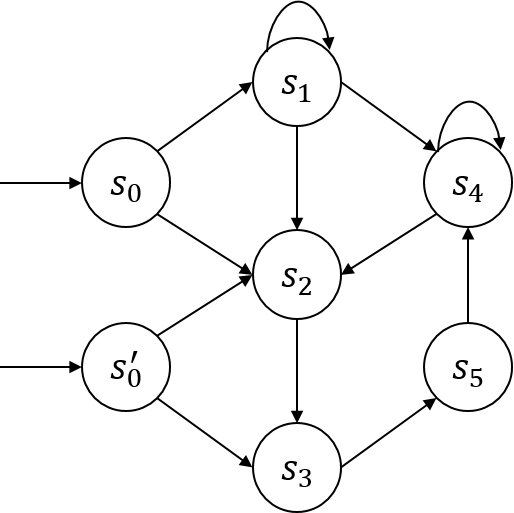
\includegraphics[scale=\figscale]{figures/transition-system.png}
        \caption{Transition system}
    \end{subfigure}
    \begin{subfigure}[b]{\subfigw}
        \centering
        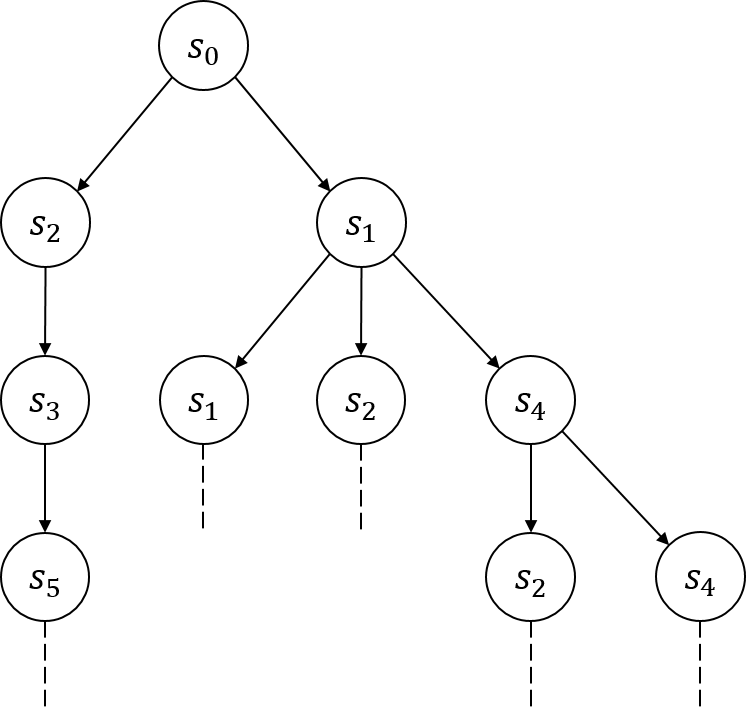
\includegraphics[scale=\figscale]{figures/ctl-interpretation.png}
        \caption{\gls{ctl} interpretation}
        \label{fig:ctl-int}
    \end{subfigure}
    \begin{subfigure}[b]{\subfigw}
        \centering
        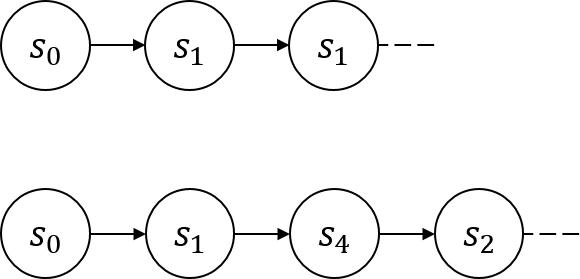
\includegraphics[scale=\figscale]{figures/ltl-interpretation.png}
        \caption{\gls{ltl} interpretation}
    \end{subfigure}
    \caption{nuXmv modules illustrated}
\end{figure}

\todo{Reference whole figure}

\gls{ltl} on the other hand is a temporal logic and as such supports the specification of properties over time.
Both, \gls{ltl} and \gls{ctl}, will be introduced semi-formally here as presented in the \citetitle{nuXmv} \cite{nuXmv}.
Interpretations and models of an \gls{ltl} formula are infinite execution paths of a system, or in the context of nuXmv.
\todo{Example}
Let $ T = (t_1, t_2, \dots) $ be such an execution path.
The most simple form of an \gls{ltl} formula again is a next-expression \smv{p}.
$ T $ models \smv{p} in \gls{ltl} if \smv{p} is true in $ t_1 $.
Furthermore, there are five main temporal operators.
\gls{ltl} formulas are defined syntactically and semantically in the usual, recursive way:
\todo{truly inductive definition}
\begin{description}
    \item[Next] \lstinline[language=smv,mathescape=true]{$ \varphi := $ X p}: $ T $ models $ \varphi $ if \smv{p} is true in $ t_2 $.
    \item[Globally] \lstinline[language=smv,mathescape=true]{$ \varphi := $ G p}: $ T $ models $ \varphi $ if \smv{p} is true for \textit{all} $ t_i $, $ 1 \leq i $.
    \item[Finally] \lstinline[language=smv,mathescape=true]{$ \varphi := $ F p}: $ T $ models $ \varphi $ if \smv{p} is true for \textit{some} $ t_i $, $ 1 \leq i $.
    \item[Until] \lstinline[language=smv,mathescape=true]{$ \varphi := $ p U p'}: $ T $ models $ \varphi $ if \smv{p} is true in $ t_1 $ to $ t_i $, $ 1 \leq i $, and at $ t_{i + 1} $, \smv{p'} is true.
    \item[Releases] \lstinline[language=smv,mathescape=true]{$ \varphi := $ p V p'}: $ T $ models $ \varphi $ if \smv{p'} holds in $ t_1 $ to $ t_i $, $ 1 \leq i $, and in $ t_i $ also \smv{p} is true.
    Alternatively, $ i $ might not be bounded, i.e. \smv{p} then is never and \smv{p'} globally true.
\end{description}

When an \gls{ltl} specification \smv{p} is checked by nuXmv, it is verified that \smv{p} is true for \textit{all} infinitely long execution paths of the transition system given by the main module.
Consequently, an invariant \smv{p} can also be expressed as the \gls{ltl} formula \smv{G p}.

Additionally, there are analogous operators for the past.
\smv{Y p} and \smv{Z p} are the past-version of \smv{X} with the distinction that \smv{Y} is false at $ t_1 $ and \smv{Z} is true at $ t_1 $.
The \enquote{Historically} operator \smv{H p} is the counterpart to \smv{G} and the \enquote{Once} operator \smv{O p} is the counterpart to \smv{F}.

\todo{Grafik für LTL}

\gls{ctl} formulas share much of the idea of \gls{ltl} formulas but they differ in the interpretations and models for formulas.
Whereas in \gls{ltl} an interpretation of a formula is a infinitely long execution path of a transition system, in \gls{ctl} an interpretation of a formula is a transition system itself or more specifically: the unwinded transition relation of a transition system as a tree (hence the name computation \textit{tree} logic).
Therefore, it is straightforward how \gls{ctl} formulas are checked by nuXmv: it is checked whether the transition system unwinded as a tree for some fixed initial state models the formula.
Again, the most simple form of a \gls{ctl} formula is a next-expression \smv{p}.
To illustrate the models-relation for \gls{ctl}, consider the example tree depicted in figure \ref{fig:ctl-int}.
Such a tree $ T $ models \smv{p} is \smv{p} is true in state $ x_0 $.

\todo{truly inductive definition}
The temporal operators supported by \gls{ctl} are the following:
\begin{description}
    \item[Exists globally] \lstinline[language=smv,mathescape=true]{$ \varphi := $ EG p}: $ T $ models $ \varphi $ if there exists an infinite path $ (x_0, \dots) $ in $ T $ such that \smv{p} is true for all $ x_i $ on the path.
    \item[Exists next state] \lstinline[language=smv,mathescape=true]{$ \varphi := $ EX p}: $ T $ models $ \varphi $ if there exists a next state $ x_i $ to $ x_0 $ such that \smv{p} is true in $ x_i $.
    \item[Exists finally] \lstinline[language=smv,mathescape=true]{$ \varphi := $ EF p}: $ T $ models $ \varphi $ if \smv{p} is true in some $ x_i $
    \item[For all globally] \lstinline[language=smv,mathescape=true]{$ \varphi := $ AG p}: $ T $ models $ \varphi $ if for all infinite paths $ (x_0, \dots) $ in $ T $, \smv{p} is true in $ x_i $.
    \item[For all next state] \lstinline[language=smv,mathescape=true]{$ \varphi := $ AX p}: $ T $ models $ \varphi $ if for all successor states $ x_i $ of $ x_0 $, \smv{p} is true in $ x_i $.
    \item[For all finally] \lstinline[language=smv,mathescape=true]{$ \varphi := $ AF p}: $ T $ models $ \varphi $ if for all infinite paths $ (x_0, \dots) $ there is any $ x_i $ such that \smv{p} is true in $ x_i $.
\end{description}

It can be seen that the most important \gls{ltl} operators \smv{X}, \smv{G} and \smv{F} are adopted to \gls{ctl} by existentially and universally quantifying each.

\begin{example}
    To illustrate the relation of \gls{ltl} and \gls{ctl} consider some module $ M $ and its transition tree $ T $ as well as the set of all execution paths $ P $.
    Now let \smv{p} be some next expression.
    One has:
    \begin{itemize}
        \item $ T $ models \smv{AG p} iff for all $ p \in P $, $ p $ models \smv{G p}
        \item $ T $ models \smv{EG} iff there exists a $ p \in P $ such that $ p $ models \smv{G p}
    \end{itemize}
    The same applies to \smv{X} and \smv{F} respectively.
    However, in general, \gls{ltl} and \gls{ctl} do not share the same expressive power and neither is strictly more expressive than the other.
\end{example}

\begin{example}
    Consider the example invariant, \gls{ltl} and \gls{ctl} specifications depicted in snippet \ref{snpt:nuxmv-spec}.
    These specify high level properties about the traffic lights example in snippet \ref{snpt:nuxmv}.

    \begin{figure}
        \begin{lstlisting}[
            language=smv,
            caption={An example of a specification in nuXmv},
            label={snpt:nuxmv-spec}
        ]
            INVARSPEC traffic_lights != ped_lights;
            LTLSPEC G (ped_button -> F ped_lights = g);
            CTLSPEC (AF traffic_lights = g) & (AF ped_lights = g);
        \end{lstlisting}
    \end{figure}


    In nuXmv, specifications are introduced by \smv{INVARSPEC}, \smv{LTLSPEC}, or \smv{LTLSPEC} and optionally may be preceded by a name which is omitted in this example.
    The invariant in the example states that at no point can the traffic and the pedestrian lights show green or red simultaneously.
    The \gls{ltl} formula specifies that whenever the button for the pedestrians is pressed, at some point the pedestrian lights must show green.
    The \gls{ctl} formula specifies that in unwindings of the transition relation, at some point the traffic lights must show green and at some point the pedestrian lights must show green.

    In this example, both the invariant and the \gls{ltl} specification are met by the model.
    The \gls{ctl} specification though is false.
    nuXmv gives the following counter-example:

    \begin{lstlisting}
        -- specification (AF traffic_lights = g & AF ped_lights = g)  is false
        -- as demonstrated by the following execution sequence
        Trace Description: CTL Counterexample
        Trace Type: Counterexample
        -> State: 1.1 <-
        ped_waiting = FALSE
        traffic_lights = g
        ped_lights = r
    \end{lstlisting}

    Counter-examples in nuXmv always show a finite fraction of an infinite execution path.
    For \gls{ltl} formulas, this fraction loops at some point thus inducing an infinite trace.
    For \gls{ctl} formulas on the other hand, the counter-example marks the longest, unambiguous path in the transition tree to a subtree that violates the formula at hand.
    Only one state being depicted in the counter-example above indicates that the computation tree with the initial state given above and in which no variable ever changes violates the \gls{ctl} formula at hand.
    This tree illustrates a world in which the button for pedestrians is never pressed and therefore, the pedestrian lights will correctly never show green.

    While it is not explicitly mentioned in the user manual how input variables relate to the states in the unwinding of the transition relation for the interpretation of a \gls{ctl} formula, it is assumed here that the input variables are not part of the state space; otherwise the counter example given above would not apply since the state where \smv{ped_button} becomes true trivially is reachable.
    This assumption is supported by the fact that in nuXmv, \gls{ctl} formulas must not reference input variables.
    In other words, this means that one must not rely on input variables when verifying a system which is completely reasonable.
\end{example}

Whereas SPIN was problematic because its input language didn't match the needs of this thesis, and SPACER or \muZ{} were problematic because there output does not match the needs of this thesis, nuXmv delivers in both aspects.
The traces generated as counter-examples serve as illustration what specifically went wrong on a property.
\todo{Example with while-loop}
The input language allows to implement modules that are limited in the description of the transition relation itself\footnote{%
    Since transitions are constrained by propositional logic and expressions without loops only, there can be issues if complex transitions should be expressed.
    For example, in section \ref{sec:ifc} we will consider a situation where for the transition of a bit vector the first bit that is high needs to be found.
    In other programming languages, one would simply iterate over all bits of the vector and break the loop on the first high bit.
    However, when constraining the transition relation, there are no loops.
    This left us with the need to implement this search for the first high bit as a sequence of nested \smv{( ? : )} expressions resembling the binary search tree for the respective bit.
} but is powerful in expressing modules as a whole.
Having variables and transition allows to implement pretty much any sequential system.
Therefore the decision was made to use nuXmv as a verification engine.

The idea for the implementation is straight-forward:
\begin{itemize}
    \item Use input variables to model instructions to the architecture
    \item Use variables to model the architectural state, i.e. registers, etc.
    \item Use transition constraints to implement the behavior of each instruction
\end{itemize}

It was furthermore decided to express the information flow control of the architecture in \gls{ltl}.
nuXmv supports a plethora of techniques to check specifications, e.g. the \citetitle{nuXmv} \cite{nuXmv} lists 47 commands to check a specification.
In the practical work for this thesis, after the decision to implement the \gls{ifc} in \gls{ltl} has been made, a couple of these techniques which apply to \gls{ltl}-checking were tested out.
In this informal evaluation it was found that the K-Liveness algorithm proposed in \cite{Claessen12} delivered best results and terminated quickly whenever the model met the specification.
Whenever this was not the case, i.e. the specification was not met by the model which was usually indicated by a long runtime of the K-Liveness algorithm, a \gls{bmc} approach computed counter-examples very efficiently.
As the technique of \gls{bmc} has already been introduced in section \ref{sec:spacer}, now, the key idea behind the K-Liveness algorithm by \citeauthor{Claessen12} shall be investigated.

In \gls{ltl} two types of properties can be distinguished: \textit{safety} and \textit{liveness} properties.
Safety properties are formulas for which every counter example has finite length.
Liveness properties on the other hand can\footnote{%
    Especially, one has that every safety property is also a liveness property but not vice versa.
} have counter-examples which are infinite and cannot be made finite.
The background of the K-Liveness algorithm is that techniques for efficiently solving safety properties already exist, i.e. the IC3 algorithm proposed in \cite{Bradley11}.
\citeauthor{Claessen12} take this algorithm and present a decision procedure for model checking liveness properties on finite state transition systems, i.e. a general algorithm for checking \gls{ltl} formulas on such systems.
The algorithm works on \gls{ltl} formulas of the canonical form: \smv{F G q} where \smv{q} is some \gls{ltl} formula.
The authors implicitly mention that any \gls{ltl} formula $ \varphi $ can be transformed into this form but give no proof or reference for this.
For such properties, \citeauthor{Claessen12} present the following lemma:
\begin{lemma}[\cite{Claessen12}]
    If a state transition system models \smv{F G q}, then there exists some integer $ k $ such that for any trace $ T $, \smv{q} is false at most $ k $ times in $ T $.
\end{lemma}
This leads to a straightforward algorithm that is sound and complete on positive instance of \gls{ltl} formulas:
\begin{enumerate}
    \item Let $ k := 0 $.
    \item Construct a formula \smv{q_new} that encodes: \smv{q} is false at most $ k $ times. \label{itm:k-live-loop}
    This obviously is a safety property.
    \item Consult the IC3 algorithm and check whether \smv{q_new} is true; if it is return that \smv{F G q} is true.
    \item Otherwise; set $ k := k + 1 $ and go to step \ref{itm:k-live-loop}.
\end{enumerate}

To have this algorithm terminate also for negative instances, i.e. where the property at hand is not modelled by the state transition system, the authors complement the basic K-Liveness algorithm with methods dedicated to finding counter-examples.
Such an algorithm needs to construct bounded counter-examples for \smv{q_new}-like properties and look for repeated states in which \smv{q} is false.
If a trace is found where such a state appears at least twice, there also is a trace in which this state occurs infinitely often thus disproving \smv{q} since no $ k $ in accordance to the lemma can be found.

\subsection{Summary \& Methodology}
\label{sec:sum-background}

The goal of this thesis is to verify a simplified version of the RISC-V \gls{isa}, MINRV8, via higher level information flow control properties.
This combines the work of \citeauthor{Reid17} \cite{Reid17} and \citeauthor{Ferraiuolo17} \cite{Ferraiuolo17}.
We adopt the requirements to these properties from \cite{Reid17}, i.e. these properties should:
\begin{displaycquote}[pp.88:2-3]{Reid17}
    \begin{itemize}
        \item express the major guarantees that programmers depend on;
        \item \textelp{be} concise so that architects can easily review and remember the entire set of properties;
        \item \textelp{be} stable so that architectural extensions don't invalidate large numbers of rules;
        \item \textelp{} describe the architecture differently from existing specification to reduce the risk of common-mode failure.
    \end{itemize}
\end{displaycquote}

To achieve this, we will investigate the RISC-V architecture in more detail and define as well as implement the MINRV8 architecture in section \ref{sec:arch}.
This architecture will stick to the \gls{risc}-properties as defined in \cite{Hennessy12} in that it will be a load-store architecture, instructions will operate on registers mainly, and there are few, homogenously encoded instructions available.
A model of this instruction set architecture will be implemented in nuXmv.

As a next step, the two terms of information flow control \textit{policy} and information flow \textit{control} will be applied to the MINRV8 architecture, thus, using the work of \citeauthor{Ferraiuolo17} \cite{Ferraiuolo17} to define higher level properties to verify the architecture against.
As a first step in section \ref{sec:checking}, it will be investigated how the policy in \cite{Ferraiuolo17} which applies to \gls{hdl} code can be carried over to \glspl{isa} and implemented in nuXmv.
By using nuXmv as a verification tool, we enhance on \cite{Reid17} in the key aspect, that unbounded numbers of transitions are taken into account.
When this has been dealt with, the actual information flow control will be expressed as \gls{ltl} properties.
These properties will assume the user-mode of the system to be compromised and express that insecure flows of information between machine- and user-mode are impossible.

The results of this verification process will be discussed in section \ref{sec:results}.
There, it will be of subject to identify either weaknesses of and respective mitigations for the MINRV8 architecture or to state rules that \gls{os} or compiler engineers must obey in order to write programs that are safe in regard to aforementioned information flow properties.

From section \ref{sec:discussion} onwards, these results will be discussed, put into context and summarized.
